\documentclass{beamer}
\usepackage[utf8]{inputenc}
\usetheme{Madrid}
\setbeamertemplate{navigation symbols}{}%remove navigation symbols
\setbeamercovered{transparent}
\usepackage[T1]{fontenc}
\usepackage{lmodern}

\settowidth{\leftmargini}{\usebeamertemplate{itemize item}}
\addtolength{\leftmargini}{\labelsep}
\addtolength{\leftmargini}{0.1cm}
\settowidth{\leftmarginii}{\usebeamertemplate{itemize item}}
\addtolength{\leftmarginii}{\labelsep}

\usepackage{listings-rust}
\lstset{
  language=Rust,
  breaklines=true,
  extendedchars=true,
  captionpos=b,
  style=boxed,
  escapechar=@,
  basicstyle=\scriptsize\ttfamily,
  % We want to disable any syntax coloring to focus on awareness colors
  stringstyle=,
  keywordstyle=,% reserved keywords
  keywordstyle=[2],% traits
  keywordstyle=[3],% primitive types
  keywordstyle=[4],% type and value constructors
  keywordstyle=[5],% macros
  aboveskip=0pt,
  belowskip=0pt,
}
\lstdefinestyle{diff}{
  morecomment=[l][\color{red}]{-},
  morecomment=[l][\color{olive}]{+},
}

\usepackage{tikz}
\usetikzlibrary{calc}
\usetikzlibrary{positioning}
\usetikzlibrary{shapes.geometric}
\tikzset{baseline=(current bounding box.center)}
\tikzstyle{varnode} = [draw, circle, text height=1.5ex, text depth=.25ex, align=center]
\tikzstyle{mvnode} = [draw, regular polygon, regular polygon sides=3, text height=1.5ex, text depth=.25ex, align=center, inner sep=2]
\tikzstyle{changenode} = [draw, rectangle, scale=0.8]
\tikzstyle{condnode} = [draw, diamond]
\tikzstyle{conflict} = [red, fill=red!10]
\tikzstyle{colorA} = [fill=blue!30]
\tikzstyle{colorB} = [fill=orange!40]
\tikzstyle{colorDel} = [fill=red!20]
\tikzstyle{colorIns} = [fill=olive!20]

\usepackage{soul}
% LaTeX purple magic to make soul compatible with beamer
\makeatletter
\let\UL\ul
\renewcommand\ul{%
  \let\set@color\beamerorig@set@color
  \let\reset@color\beamerorig@reset@color
  \UL}
\let\ST\st
\renewcommand\st{%
  \let\set@color\beamerorig@set@color
  \let\reset@color\beamerorig@reset@color
  \ST}
\let\HL\hl
\renewcommand\hl{%
  \let\set@color\beamerorig@set@color
  \let\reset@color\beamerorig@reset@color
  \HL}
\makeatother

\usepackage{bussproofs}
\usepackage{amsmath}
\usepackage{amssymb}
\newcommand\typsep{\mathrel{|}}
\newcommand\merge{\mathbin{\Join}}
\newcommand\mathst[1]{\text{\st{$#1$}}}
\newcommand\mathul[1]{\text{\ul{$#1$}}}
\newcommand\black[1]{\text{\sethlcolor{black}\color{white}\hl{$#1$}}}
\newcommand\id{\square}
\newcommand\change[2]{\mathst{#1} \rightarrow \mathul{#2}}
\DeclareMathOperator\InsConflict{Ins!}
\DeclareMathOperator\DelConflict{Del!}
\DeclareMathOperator\OrdConflict{Ord!}
\DeclareMathOperator\MvConflict{Mv!}
\DeclareMathOperator\dom{dom}
\newcommand\rtstate[3]{\langle #1, #2, #3\rangle}
\newcommand\vrtstate[3]{\left\langle\begin{matrix}#1,\\#2,\\#3\end{matrix}\right\rangle}
\allowdisplaybreaks

\newcommand{\sectiontitleframe}{
    \begin{frame}
        \vfill
        \centering
        \begin{beamercolorbox}[sep=8pt,center,shadow=true,rounded=true]{title}
            \usebeamerfont{title}\insertsectionhead\par%
        \end{beamercolorbox}
        \vfill
\end{frame}}

\pdfstringdefDisableCommands{\def\\{}}

\title{Semantically checked source code merge}
\author[Guillaume Bertholon]{Guillaume Bertholon\\ supervised by Yann Régis Gianas}
\institute[IRIF]{IRIF -- Université de Paris}
\date[MPRI internship -- 2020]{MPRI internship\\
March 9 -- July 24, 2020}

\begin{document}

\begin{frame}
 \maketitle
\end{frame}

\begin{frame}[fragile]{Merging program modifications}
\begin{columns}
\begin{column}<2,4>{0.33\textwidth}
\center{\color{blue}Blue commit}
\vspace{0.5em}
\begin{lstlisting}[rulecolor=\color{blue!20}]
fn f(c: bool) -> i32 {
    let x = answer();
    let y = if c {
        2
    } else {
        x * x
    };
    x / y
}

fn answer() -> i32 {
    let a = 2;
    let b = 40;
    a + b
}
\end{lstlisting}
\end{column}
\begin{column}{0.33\textwidth}
\center{Original}
\vspace{0.5em}
\begin{lstlisting}
fn f(c: bool) -> i32 {
    let a = 2;
    let b = 40;
    let x = a + b;

    let y = if c {
        2
    } else {
        x
    };
    x * y
}
\end{lstlisting}
\end{column}
\begin{column}<3->{0.33\textwidth}
\center{\color{orange}Orange commit}
\vspace{0.5em}
\begin{lstlisting}[rulecolor=\color{orange!30}]
fn f(c: bool) -> i32 {
    let a = 4;
    let b = 41;
    let x = a + b;

    let y = if c {
        0
    } else {
        x
    };
    x * y
}
\end{lstlisting}
\end{column}
\end{columns}

\begin{alertblock}<4>{Question}
How can we merge both commits into a working program?
\end{alertblock}

\end{frame}

\begin{frame}[fragile]{Merging program modifications: Standard approach (Git)}
\vspace{-0.5em}
\begin{columns}
\begin{column}{0.5\textwidth}
\center{\color{blue}Blue difference}
\vspace{0.5em}
\begin{lstlisting}[style=diff,rulecolor=\color{blue!20}]
 fn f(c: bool) @-@> i32 {
-    let a = 2;
-    let b = 40;
-    let x = a + b;
-
+    let x = answer();
     let y = if c {
         2
     } else {
-        x
+        x * x
     };
-    x * y
+    x / y
+}
+
+fn answer() -> i32 {
+    let a = 2;
+    let b = 40;
+    a + b
 }
\end{lstlisting}
\end{column}
\begin{column}{0.5\textwidth}
\center{\color{orange}Orange difference}
\vspace{0.5em}
\begin{lstlisting}[style=diff,rulecolor=\color{orange!30}]
 fn f(c: bool) @-@> i32 {
-    let a = 2;
-    let b = 40;
+    let a = 4;
+    let b = 41;
     let x = a @+@ b;
 
     let y = if c {
-        2
+        0
     } else {
         x
     };
     x * y
 }
\end{lstlisting}
\end{column}
\end{columns}
\end{frame}

\begin{frame}[fragile]{Merging program modifications: Standard approach (Git)}
\vspace{-1em}
\begin{columns}
\begin{column}{0.4\textwidth}
\center{Merged version}
\vspace{0.5em}
\begin{lstlisting}
 fn f(c: bool) -> i32 {
<<<<<<< Blue commit
    @\color{blue}let x = answer();@
=======
    @\color{orange}let a = 4;@
    @\color{orange}let b = 41;@
    let x = a + b;

>>>>>>> Orange commit
    let y = if c {
        @\color{orange}0@
    } else {
        @\color{blue}x * x@
    };
    @\color{blue}x / y@
}

@\color{blue}fn answer() -> i32 \{@
    @\color{blue}let a = 2;@
    @\color{blue}let b = 40;@
    @\color{blue}a + b@
@\color{blue}\}@
\end{lstlisting}
\end{column}
\begin{column}{0.55\textwidth}
\begin{block}<2->{Problems}
\begin{itemize}
 \item<2-> Lines do not cary any semantics: code style matters
 \item<3-> Refactorings create conflicts
 \item<4-> Bugs can be silently introduced by fusion itself:
 the blue modification (l.15) rely on an invariant broken by orange (l.11).
\end{itemize}
\end{block}
\begin{alertblock}<5>{Question}
Can we design a merging procedure preserving the semantics of both modifications ?
\end{alertblock}
\end{column}
\end{columns}
\end{frame}

\begin{frame}{Divide the problem into two phases}
\begin{alertblock}{A difficult problem}
\begin{itemize}
 \item Semantically compare two programs is hard
 \item We need a way to align executions and program modifications
\end{itemize}
\end{alertblock}
\begin{columns}
\begin{column}{0.45\textwidth}
\begin{block}<2->{Syntactic fusion}
\begin{itemize}
 \item Align changes by syntax
 \item Difference then fusion
 \item Keep provenance anotations
\end{itemize}
\end{block}
\end{column}
\begin{column}{0.45\textwidth}
\begin{block}<3->{Semantic check}
\begin{itemize}
 \item Check that changes do not rely on broken invariants from other commits
 \item Force the user to resolve semantic ambiguities
\end{itemize}
\end{block}
\end{column}
\end{columns}
\end{frame}

\section{Syntactic difference}
\sectiontitleframe

\begin{frame}{Computing syntactic difference: Spine alignment}
\centering
\begin{onlyenv}<1>
$$\change{\{ \mathbf{let}\ x = 3;\ y = x \}}{\{ y = 5;\ z = 9 \}}$$

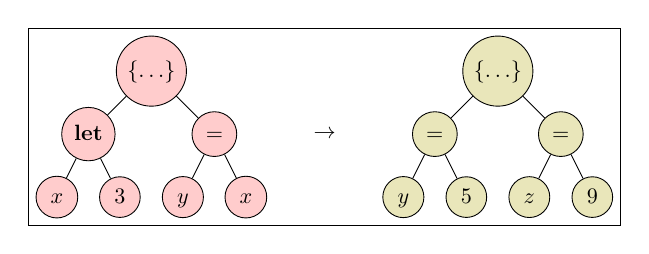
\begin{tikzpicture}
\node[changenode] (change) {\tikz{
    \node[varnode, colorDel] (del_block) {$\{\ldots\}$};
    \node[varnode, colorDel] (del_stmt1) at ($(del_block)+(-1,-1)$) {$\textbf{let}$};
    \node[varnode, colorDel] (del_stmt2) at ($(del_block)+(1,-1)$) {$=$};
    \node[varnode, colorDel] (del_x) at ($(del_stmt1)+(-0.5,-1)$) {$x$};
    \node[varnode, colorDel] (del_three) at ($(del_stmt1)+(0.5,-1)$) {$3$};
    \node[varnode, colorDel] (del_y) at ($(del_stmt2)+(-0.5,-1)$) {$y$};
    \node[varnode, colorDel] (del_yx) at ($(del_stmt2)+(0.5,-1)$) {$x$};
    \draw (del_block) -- (del_stmt1);
    \draw (del_block) -- (del_stmt2);
    \draw (del_stmt1) -- (del_x);
    \draw (del_stmt1) -- (del_three);
    \draw (del_stmt2) -- (del_y);
    \draw (del_stmt2) -- (del_yx);

    \node[varnode, colorIns] (ins_block) at ($(del_block)+(5.5,0)$) {$\{\ldots\}$};
    \node[varnode, colorIns] (ins_stmt1) at ($(ins_block)+(-1,-1)$) {$=$};
    \node[varnode, colorIns] (ins_stmt2) at ($(ins_block)+(1,-1)$) {$=$};
    \node[varnode, colorIns] (ins_y) at ($(ins_stmt1)+(-0.5,-1)$) {$y$};
    \node[varnode, colorIns] (ins_five) at ($(ins_stmt1)+(0.5,-1)$) {$5$};
    \node[varnode, colorIns] (ins_z) at ($(ins_stmt2)+(-0.5,-1)$) {$z$};
    \node[varnode, colorIns] (ins_nine) at ($(ins_stmt2)+(0.5,-1)$) {$9$};
    \draw (ins_block) -- (ins_stmt1);
    \draw (ins_block) -- (ins_stmt2);
    \draw (ins_stmt1) -- (ins_y);
    \draw (ins_stmt1) -- (ins_five);
    \draw (ins_stmt2) -- (ins_z);
    \draw (ins_stmt2) -- (ins_nine);

    \node (arrow) at ($(del_stmt2)!0.5!(ins_stmt1)$) {$\rightarrow$};
}};
\end{tikzpicture}
\end{onlyenv}

\begin{onlyenv}<2>
$$\{\change{\mathbf{let}\ x = 3;\ y = x}{y = 5;\ z = 9}\}$$

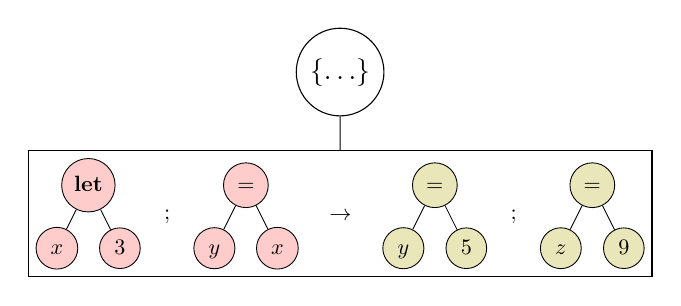
\begin{tikzpicture}
\node[varnode] (spine_block) {$\{\ldots\}$};
\node[changenode] (change) at ($(spine_block)+(0,-1.8)$) {\tikz{
    \node[varnode, colorDel] (del_stmt1)  {$\textbf{let}$};
    \node[varnode, colorDel] (del_stmt2) at ($(del_stmt1)+(2.5,0)$) {$=$};
    \node[varnode, colorDel] (del_x) at ($(del_stmt1)+(-0.5,-1)$) {$x$};
    \node[varnode, colorDel] (del_three) at ($(del_stmt1)+(0.5,-1)$) {$3$};
    \node[varnode, colorDel] (del_y) at ($(del_stmt2)+(-0.5,-1)$) {$y$};
    \node[varnode, colorDel] (del_yx) at ($(del_stmt2)+(0.5,-1)$) {$x$};
    \draw (del_stmt1) -- (del_x);
    \draw (del_stmt1) -- (del_three);
    \draw (del_stmt2) -- (del_y);
    \draw (del_stmt2) -- (del_yx);

    \node[varnode, colorIns] (ins_stmt1) at ($(del_stmt2)+(3,0)$) {$=$};
    \node[varnode, colorIns] (ins_stmt2) at ($(ins_stmt1)+(2.5,0)$) {$=$};
    \node[varnode, colorIns] (ins_y) at ($(ins_stmt1)+(-0.5,-1)$) {$y$};
    \node[varnode, colorIns] (ins_five) at ($(ins_stmt1)+(0.5,-1)$) {$5$};
    \node[varnode, colorIns] (ins_z) at ($(ins_stmt2)+(-0.5,-1)$) {$z$};
    \node[varnode, colorIns] (ins_nine) at ($(ins_stmt2)+(0.5,-1)$) {$9$};
    \draw (ins_stmt1) -- (ins_y);
    \draw (ins_stmt1) -- (ins_five);
    \draw (ins_stmt2) -- (ins_z);
    \draw (ins_stmt2) -- (ins_nine);

    \node (arrow) at ($($(del_stmt2)!0.5!(del_yx)$)!0.5!($(ins_stmt1)!0.5!(ins_y)$)$) {$\rightarrow$};
    \node (del_semicolon) at ($($(del_stmt2)!0.5!(del_yx)$)!0.5!($(del_stmt1)!0.5!(del_x)$)$) {;};
    \node (ins_semicolon) at ($($(ins_stmt2)!0.5!(ins_nine)$)!0.5!($(ins_stmt1)!0.5!(ins_y)$)$) {;};
}};
\draw (spine_block) -- (change);
\end{tikzpicture}
\end{onlyenv}

\begin{onlyenv}<3>
$$\{\mathst{\mathbf{let}\ x = 3;}\ (\change{y = x}{y = 5;\ z = 9})\}$$

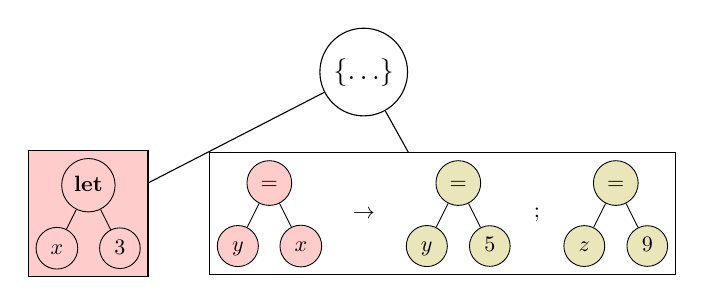
\begin{tikzpicture}
\node[varnode] (spine_block) {$\{\ldots\}$};
\node[changenode, colorDel] (spine_stmt1) at ($(spine_block)+(-3.5,-1.8)$) {\tikz{
    \node[varnode] (del_stmt) {$\textbf{let}$};
    \node[varnode] (del_x) at ($(del_stmt)+(-0.5,-1)$) {$x$};
    \node[varnode] (del_three) at ($(del_stmt)+(0.5,-1)$) {$3$};
    \draw (del_stmt) -- (del_x);
    \draw (del_stmt) -- (del_three);
}};
\node[changenode] (change) at ($(spine_block)+(1,-1.8)$) {\tikz{
    \node[varnode, colorDel] (del_stmt2) {$=$};
    \node[varnode, colorDel] (del_y) at ($(del_stmt2)+(-0.5,-1)$) {$y$};
    \node[varnode, colorDel] (del_yx) at ($(del_stmt2)+(0.5,-1)$) {$x$};
    \draw (del_stmt2) -- (del_y);
    \draw (del_stmt2) -- (del_yx);

    \node[varnode, colorIns] (ins_stmt1) at ($(del_stmt2)+(3,0)$) {$=$};
    \node[varnode, colorIns] (ins_stmt2) at ($(ins_stmt1)+(2.5,0)$) {$=$};
    \node[varnode, colorIns] (ins_y) at ($(ins_stmt1)+(-0.5,-1)$) {$y$};
    \node[varnode, colorIns] (ins_five) at ($(ins_stmt1)+(0.5,-1)$) {$5$};
    \node[varnode, colorIns] (ins_z) at ($(ins_stmt2)+(-0.5,-1)$) {$z$};
    \node[varnode, colorIns] (ins_nine) at ($(ins_stmt2)+(0.5,-1)$) {$9$};
    \draw (ins_stmt1) -- (ins_y);
    \draw (ins_stmt1) -- (ins_five);
    \draw (ins_stmt2) -- (ins_z);
    \draw (ins_stmt2) -- (ins_nine);

    \node (arrow) at ($($(del_stmt2)!0.5!(del_yx)$)!0.5!($(ins_stmt1)!0.5!(ins_y)$)$) {$\rightarrow$};
    \node (ins_semicolon) at ($($(ins_stmt2)!0.5!(ins_nine)$)!0.5!($(ins_stmt1)!0.5!(ins_y)$)$) {;};
}};
\draw (spine_block) -- (spine_stmt1);
\draw (spine_block) -- (change);
\end{tikzpicture}
\end{onlyenv}

\begin{onlyenv}<4>
$$\{\mathst{\mathbf{let}\ x = 3;}\ \change{y = x}{y = 5};\ (\change{[]}{z = 9})\}$$

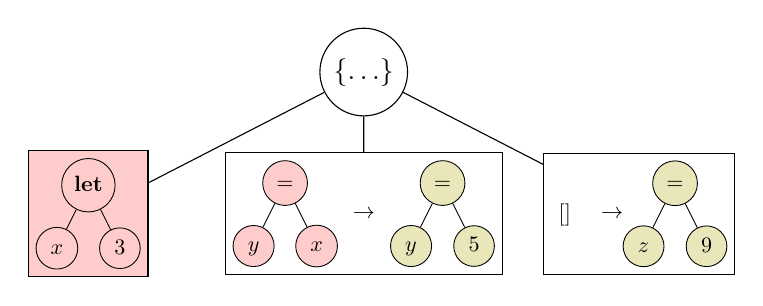
\begin{tikzpicture}
\node[varnode] (spine_block) {$\{\ldots\}$};
\node[changenode, colorDel] (spine_stmt1) at ($(spine_block)+(-3.5,-1.8)$) {\tikz{
    \node[varnode] (del_stmt) {$\textbf{let}$};
    \node[varnode] (del_x) at ($(del_stmt)+(-0.5,-1)$) {$x$};
    \node[varnode] (del_three) at ($(del_stmt)+(0.5,-1)$) {$3$};
    \draw (del_stmt) -- (del_x);
    \draw (del_stmt) -- (del_three);
}};
\node[changenode] (change) at ($(spine_block)+(0,-1.8)$) {\tikz{
    \node[varnode, colorDel] (del_stmt2) {$=$};
    \node[varnode, colorDel] (del_y) at ($(del_stmt2)+(-0.5,-1)$) {$y$};
    \node[varnode, colorDel] (del_yx) at ($(del_stmt2)+(0.5,-1)$) {$x$};
    \draw (del_stmt2) -- (del_y);
    \draw (del_stmt2) -- (del_yx);

    \node[varnode, colorIns] (ins_stmt1) at ($(del_stmt2)+(2.5,0)$) {$=$};
    \node[varnode, colorIns] (ins_y) at ($(ins_stmt1)+(-0.5,-1)$) {$y$};
    \node[varnode, colorIns] (ins_five) at ($(ins_stmt1)+(0.5,-1)$) {$5$};
    \draw (ins_stmt1) -- (ins_y);
    \draw (ins_stmt1) -- (ins_five);

    \node (arrow) at ($($(del_stmt2)!0.5!(del_yx)$)!0.5!($(ins_stmt1)!0.5!(ins_y)$)$) {$\rightarrow$};
}};
\node[changenode] (rest) at ($(spine_block)+(3.5,-1.8)$) {\tikz{
    \node[varnode, colorIns] (ins_stmt2) {$=$};
    \node[varnode, colorIns] (ins_z) at ($(ins_stmt2)+(-0.5,-1)$) {$z$};
    \node[varnode, colorIns] (ins_nine) at ($(ins_stmt2)+(0.5,-1)$) {$9$};

    \node (del_empty) at ($($(ins_stmt2)!0.5!(ins_z)$)+(-1.5,0)$) {[]};
    
    \draw (ins_stmt2) -- (ins_z);
    \draw (ins_stmt2) -- (ins_nine);
    
    \node (arrow) at ($(del_empty)!0.5!($(ins_stmt2)!0.5!(ins_z)$)$) {$\rightarrow$};

}};
\draw (spine_block) -- (spine_stmt1);
\draw (spine_block) -- (change);
\draw (spine_block) -- (rest);
\end{tikzpicture}
\end{onlyenv}

\begin{onlyenv}<5>
$$\{\mathst{\mathbf{let}\ x = 3;}\ y = \change{x}{5};\ (\change{[]}{z = 9})\}$$

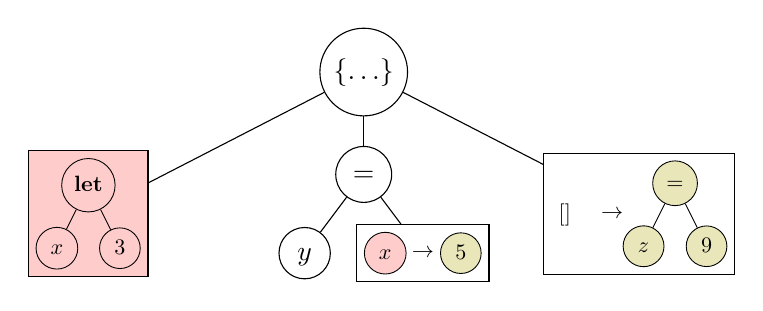
\begin{tikzpicture}
    \node[varnode] (spine_block) {$\{\ldots\}$};
    \node[changenode, colorDel] (spine_stmt1) at ($(spine_block)+(-3.5,-1.8)$) {\tikz{
        \node[varnode] (del_stmt) {$\textbf{let}$};
        \node[varnode] (del_x) at ($(del_stmt)+(-0.5,-1)$) {$x$};
        \node[varnode] (del_three) at ($(del_stmt)+(0.5,-1)$) {$3$};
        \draw (del_stmt) -- (del_x);
        \draw (del_stmt) -- (del_three);
    }};
    \node[varnode] (spine_stmt2) at ($(spine_block)+(0,-1.3)$) {$=$};
    \node[changenode] (rest) at ($(spine_block)+(3.5,-1.8)$) {\tikz{
        \node[varnode, colorIns] (ins_stmt2) {$=$};
        \node[varnode, colorIns] (ins_z) at ($(ins_stmt2)+(-0.5,-1)$) {$z$};
        \node[varnode, colorIns] (ins_nine) at ($(ins_stmt2)+(0.5,-1)$) {$9$};

        \node (del_empty) at ($($(ins_stmt2)!0.5!(ins_z)$)+(-1.5,0)$) {[]};
        
        \draw (ins_stmt2) -- (ins_z);
        \draw (ins_stmt2) -- (ins_nine);
        
        \node (arrow) at ($(del_empty)!0.5!($(ins_stmt2)!0.5!(ins_z)$)$) {$\rightarrow$};
    }};{};
    \node[varnode] (spine_y) at ($(spine_stmt2)+(-0.75,-1)$) {$y$};
    \node[changenode] (change_y) at ($(spine_stmt2)+(0.75,-1)$) {\tikz{
        \node[varnode, colorDel] (x) {$x$};
        \node[varnode, colorIns] (five) at ($(x)+(1.2,0)$) {$5$};
        \node (arrow) at ($(x)!0.5!(five)$) {$\rightarrow$};
    }};
    \draw (spine_block) -- (spine_stmt1);
    \draw (spine_block) -- (spine_stmt2);
    \draw (spine_block) -- (rest);
    \draw (spine_stmt2) -- (spine_y);
    \draw (spine_stmt2) -- (change_y);
\end{tikzpicture}
\end{onlyenv}

\begin{onlyenv}<6->
$$\{\mathst{\mathbf{let}\ x = 3;}\ y = \change{x}{5};\ \mathul{z = 9}\}$$

\begin{tikzpicture}
    \node[varnode] (spine_block) {$\{\ldots\}$};
    \node[changenode, colorDel] (spine_stmt1) at ($(spine_block)+(-3.5,-1.8)$) {\tikz{
        \node[varnode] (del_stmt) {$\textbf{let}$};
        \node[varnode] (del_x) at ($(del_stmt)+(-0.5,-1)$) {$x$};
        \node[varnode] (del_three) at ($(del_stmt)+(0.5,-1)$) {$3$};
        \draw (del_stmt) -- (del_x);
        \draw (del_stmt) -- (del_three);
    }};
    \node[varnode] (spine_stmt2) at ($(spine_block)+(0,-1.3)$) {$=$};
    \node[changenode, colorIns] (spine_stmt3) at ($(spine_block)+(3.5,-1.8)$) {\tikz{
        \node[varnode] (ins_stmt) at ($(ins_block)+(1,-1)$) {$=$};
        \node[varnode] (ins_z) at ($(ins_stmt)+(-0.5,-1)$) {$z$};
        \node[varnode] (ins_nine) at ($(ins_stmt)+(0.5,-1)$) {$9$};
        \draw (ins_stmt) -- (ins_z);
        \draw (ins_stmt) -- (ins_nine);
    }};{};
    \node[varnode] (spine_y) at ($(spine_stmt2)+(-0.75,-1)$) {$y$};
    \node[changenode] (change_y) at ($(spine_stmt2)+(0.75,-1)$) {\tikz{
        \node[varnode, colorDel] (x) {$x$};
        \node[varnode, colorIns] (five) at ($(x)+(1.2,0)$) {$5$};
        \node (arrow) at ($(x)!0.5!(five)$) {$\rightarrow$};
    }};
    \draw (spine_block) -- (spine_stmt1);
    \draw (spine_block) -- (spine_stmt2);
    \draw (spine_block) -- (spine_stmt3);
    \draw (spine_stmt2) -- (spine_y);
    \draw (spine_stmt2) -- (change_y);
\end{tikzpicture}
\end{onlyenv}

\begin{onlyenv}<7>
\vfill
Multiple possibilities: Maximize the number of shared nodes
\end{onlyenv}

\end{frame}

\begin{frame}{Computing syntactic difference: Meta-variable ellision}
\centering
\begin{onlyenv}<1-2>
$$\change{(2*x)+x}{f((2*x)-x, 2*x)}$$

\alt<2>{\tikzstyle{colorA*} = [colorA]}{\tikzstyle{colorA*} = []}
\alt<2>{\tikzstyle{colorB*} = [colorB]}{\tikzstyle{colorB*} = []}
$$\begin{tikzpicture}
    \node[varnode] (del_plus) {$+$};
    \node[varnode, colorA*] (del_times) at ($(del_plus)+(-0.7,-1)$) {$*$};
    \node[varnode, colorB*] (del_one) at ($(del_plus)+(0.7,-1)$) {$x$};
    \node[varnode, colorA*] (del_two) at ($(del_times)+(-0.5,-1)$) {$2$};
    \node[varnode, colorA*] (del_three) at ($(del_times)+(0.5,-1)$) {$x$};
    \draw (del_plus) -- (del_times);
    \draw (del_plus) -- (del_one);
    \draw (del_times) -- (del_two);
    \draw (del_times) -- (del_three);
\end{tikzpicture}
\ \ \rightarrow\ \ 
\begin{tikzpicture}
    \node[varnode] (ins_f) {$f(...)$};
    \node[varnode] (ins_minus) at ($(ins_f)+(-1.2,-1)$) {$-$};
    \node[varnode, colorA*] (ins_times) at ($(ins_minus)+(-0.7,-1)$) {$*$};
    \node[varnode, colorB*] (ins_one) at ($(ins_minus)+(0.7,-1)$) {$x$};
    \node[varnode, colorA*] (ins_two) at ($(ins_times)+(-0.5,-1)$) {$2$};
    \node[varnode, colorA*] (ins_three) at ($(ins_times)+(0.5,-1)$) {$x$};
    
    \node[varnode, colorA*] (ins_times2) at ($(ins_f)+(1.2,-1)$) {$*$};
    \node[varnode, colorA*] (ins_two2) at ($(ins_times2)+(-0.5,-1)$) {$2$};
    \node[varnode, colorA*] (ins_three2) at ($(ins_times2)+(0.5,-1)$) {$x$};

    \draw (ins_f) -- (ins_minus);
    \draw (ins_f) -- (ins_times2);
    \draw (ins_minus) -- (ins_times);
    \draw (ins_minus) -- (ins_one);
    \draw (ins_times) -- (ins_two);
    \draw (ins_times) -- (ins_three);
    \draw (ins_times2) -- (ins_two2);
    \draw (ins_times2) -- (ins_three2);
\end{tikzpicture}$$
\end{onlyenv}
\begin{onlyenv}<3>
\alt<3>{$$\change{\alpha+\beta}{f(\alpha-\beta, \alpha)}$$}{$$\change{f(\alpha-\beta, \alpha)}{\alpha+\beta}$$}

$$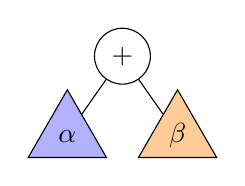
\begin{tikzpicture}
    \node[varnode] (del_plus) {$+$};
    \node[mvnode, colorA] (del_alpha) at ($(del_plus)+(-0.7,-1)$) {$\alpha$};
    \node[mvnode, colorB] (del_beta) at ($(del_plus)+(0.7,-1)$) {$\beta$};
    
    \draw (del_plus) -- (del_alpha);
    \draw (del_plus) -- (del_beta);
\end{tikzpicture}
\ \ \alt<3>{\rightarrow}{\leftarrow}\ \ 
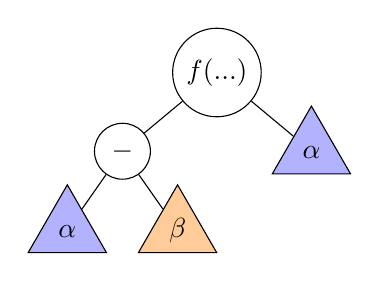
\begin{tikzpicture}
    \node[varnode] (ins_f) {$f(...)$};
    \node[varnode] (ins_minus) at ($(ins_f)+(-1.2,-1)$) {$-$};
    \node[mvnode, colorA] (ins_alpha) at ($(ins_minus)+(-0.7,-1)$) {$\alpha$};
    \node[mvnode, colorB] (ins_beta) at ($(ins_minus)+(0.7,-1)$) {$\beta$};
    \node[mvnode, colorA] (ins_alpha2) at ($(ins_f)+(1.2,-1)$) {$\alpha$};
    
    \draw (ins_f) -- (ins_minus);
    \draw (ins_f) -- (ins_alpha2);
    \draw (ins_minus) -- (ins_alpha);
    \draw (ins_minus) -- (ins_beta);
\end{tikzpicture}$$
\end{onlyenv}
\end{frame}

\begin{frame}[fragile]{Computing syntactic difference: Example}
\setstcolor{blue}
\setulcolor{blue}
\newbox\boxsemicolon
\sbox\boxsemicolon{\color{blue}\scriptsize\ttfamily;}

\begin{onlyenv}<1>
\begin{columns}
\begin{column}{0.45\textwidth}
\center{Original}
\vspace{0.5em}
\begin{lstlisting}
fn f(c: bool) -> i32 {
    let a = 2;
    let b = 40;
    let x = a + b;

    let y = if c {
        2
    } else {
        x
    };
    x * y
}
\end{lstlisting}
\end{column}
\begin{column}{0.45\textwidth}
\center{\color{blue}Blue commit}
\vspace{0.5em}
\begin{lstlisting}[rulecolor=\color{blue!40}]
fn f(c: bool) -> i32 {
    let x = answer();
    let y = if c {
        2
    } else {
        x * x
    };
    x / y
}

fn answer() -> i32 {
    let a = 2;
    let b = 40;
    a + b
}
\end{lstlisting}
\end{column}
\end{columns}
\end{onlyenv}

\begin{onlyenv}<2>
\begin{columns}
\begin{column}{0.45\textwidth}
\center{Original}
\vspace{0.5em}
\begin{lstlisting}
fn f(c: bool) -> i32 {
    @$\alpha$@;
    @$\beta$@;
    let x = @$\gamma$@;

    let y = if @$\zeta$@ {
        @$\eta$@
    } else {
        @$\delta$@
    };
    @$\delta$@ * @$\epsilon$@
}
\end{lstlisting}
\end{column}
\begin{column}{0.45\textwidth}
\center{\color{blue}Blue commit}
\vspace{0.5em}
\begin{lstlisting}[rulecolor=\color{blue!40}]
fn f(c: bool) -> i32 {
    let x = answer();
    let y = if @$\zeta$@ {
        @$\eta$@
    } else {
        @$\delta$@ * @$\delta$@
    };
    @$\delta$@ / @$\epsilon$@
}

fn answer() -> i32 {
    @$\alpha$@;
    @$\beta$@;
    @$\gamma$@
}
\end{lstlisting}
\end{column}
\end{columns}
\end{onlyenv}

\begin{onlyenv}<3>
\begin{columns}
\begin{column}{0.33\textwidth}
\center{Original}
\vspace{0.5em}
\begin{lstlisting}
fn f(c: bool) -> i32 {
    @$\alpha$@;
    @$\beta$@;
    let x = @$\gamma$@;

    let y = if @$\zeta$@ {
        @$\eta$@
    } else {
        @$\delta$@
    };
    @$\delta$@ * @$\epsilon$@
}





@@
\end{lstlisting}
\end{column}
\begin{column}{0.33\textwidth}
\center{\color{blue}Blue difference}
\vspace{0.5em}
\begin{lstlisting}[rulecolor=\color{blue!20}]
fn f(c: bool) -> i32 {
    @\st{$\alpha$;}@
    @\st{$\beta$;}@
    let x = @\st{$\gamma$} $\rightarrow$@
        @{\color{blue}\ul{answer()}}@;
    let y = if @$\id$@ {
        @$\id$@;
    } else {
        @\st{$\delta$} $\rightarrow$ \ul{$\delta$ {\color{blue}*} $\delta$}@
    };
    @\st{$\delta$ * $\epsilon$} $\rightarrow$ \ul{$\delta$ {\color{blue}/} $\epsilon$}@
}

@{\color{blue} \ul{fn answer() -> i32 \{}}@
    @\ul{$\alpha${\usebox\boxsemicolon}}@
    @\ul{$\beta${\usebox\boxsemicolon}}@
    @\ul{$\gamma$}@
@{\color{blue} \ul{\}}}@
\end{lstlisting}
\end{column}
\begin{column}{0.33\textwidth}
\center{\color{blue}Blue commit}
\vspace{0.5em}
\begin{lstlisting}[rulecolor=\color{blue!40}]
fn f(c: bool) -> i32 {


    let x = answer();
    
    let y = if @$\zeta$@ {
        @$\eta$@
    } else {
        @$\delta$@ * @$\delta$@
    };
    @$\delta$@ / @$\epsilon$@
}

fn answer() -> i32 {
    @$\alpha$@;
    @$\beta$@;
    @$\gamma$@
}
\end{lstlisting}
\end{column}
\end{columns}
\end{onlyenv}
\end{frame}

\section{Syntactic fusion}
\sectiontitleframe

\begin{frame}{Awareness colors}
\begin{block}{Base ideas}
\begin{itemize}
 \item Each commit has an tint $t \in \mathbb{T}$
 \item Each node in difference tree has a color $c \in \mathcal{P}(\mathbb{T})$
 \item Colors are used to taint values produced by a modification
\end{itemize}
\end{block}
\begin{columns}
\begin{column}{0.48\textwidth}
\setbeamercolor{block title}{bg=gray!20,fg=black}
\setbeamercolor{block body}{bg=gray!5,fg=black}
\begin{block}<2->{White color ($\top$)}
\setbeamercolor{local structure}{fg=gray!70}
\begin{itemize}
 \item Represent consensus
 \item Used for unchanged code
\end{itemize}
\end{block}
\end{column}
\begin{column}{0.48\textwidth}
\setbeamercolor{block title}{bg=black,fg=white}
\begin{block}<2->{Black color ($\bot$)}
\setbeamercolor{local structure}{fg=black}
\begin{itemize}
 \item Represent unexpected behaviour
 \item Used for semantic ambiguities
\end{itemize}
\end{block}
\end{column}
\end{columns}
\begin{block}<3->{Color composition}
\newbox\boxdelinner
\sbox\boxdelinner{\setulcolor{blue}\setul{-.75ex}{}$\mathul{x}^{\color{blue}c}$}
\newbox\boxinsinner
\sbox\boxinsinner{\setulcolor{blue}\setul{.1ex}{}$\mathul{x}^{\color{blue}c}$}
\begin{itemize}
 \item Deletion $\Rightarrow$ color union: $\setulcolor{orange}\setul{-.4ex}{}\mathul{\usebox\boxdelinner}^{\color{orange}c'} = \mathst{x}^{{\color{blue}c} \cup {\color{orange}c'}}$
 \item Insertion $\Rightarrow$ color intersection: $\setulcolor{orange}\setul{.4ex}{}\mathul{\usebox\boxinsinner}^{\color{orange}c'} = \setulcolor{black}\mathul{x}^{{\color{blue}c} \cap {\color{orange}c'}}$
\end{itemize}
\end{block}
\end{frame}

\begin{frame}{Merging syntactic differences: Merge following syntax}
\centering
\begin{onlyenv}<1-2>
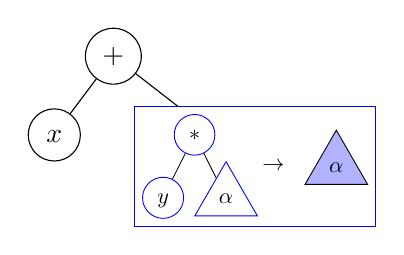
\begin{tikzpicture}
\node[varnode] (plus) {$+$};
\node[varnode] (x) at ($(plus)+(-0.75,-1)$) {$x$};
\node[changenode, color=blue] (change) at ($(plus)+(1.8,-1.4)$) {\tikz[color=black]{
    \node[varnode, color=blue] (del_times) {$\color{black}*$};
    \node[varnode, color=blue] (del_y) at ($(del_times)+(-0.5,-1)$) {$\color{black}y$};
    \node[mvnode, color=blue] (del_alpha) at ($(del_times)+(0.5,-1)$) {$\color{black}\alpha$};
    \draw (del_times) -- (del_y);
    \draw (del_times) -- (del_alpha);
    
    \node[mvnode, colorA] (ins_alpha) at ($(del_times)!0.5!(del_alpha)+(2, 0)$) {$\alpha$};
    \node (arrow) at ($(del_times)!0.5!(del_alpha)!0.5!(ins_alpha)$) {$\rightarrow$};
}};
\draw (plus) -- (x);
\draw (plus) -- (change);
\end{tikzpicture}
$\merge$
\begin{onlyenv}<1>
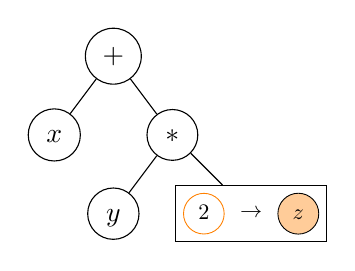
\begin{tikzpicture}
\node[varnode] (plus) {$+$};
\node[varnode] (x) at ($(plus)+(-0.75,-1)$) {$x$};
\node[varnode] (times) at ($(plus)+(0.75,-1)$) {$*$};
\node[varnode] (y) at ($(times)+(-0.75,-1)$) {$y$};
\node[changenode] (change) at ($(times)+(1,-1)$) {\tikz{
    \node[varnode, color=orange] (two) {$\color{black}2$};
    \node[varnode, colorB] (z) at ($(two)+(1.5, 0)$) {$z$};
    \node (arrow) at ($(two)!0.5!(z)$) {$\rightarrow$};
}};
\draw (plus) -- (x);
\draw (plus) -- (times);
\draw (times) -- (y);
\draw (times) -- (change);
\end{tikzpicture}
\end{onlyenv}
\begin{onlyenv}<2>
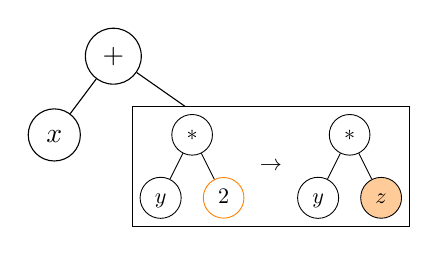
\begin{tikzpicture}
\node[varnode] (plus) {$+$};
\node[varnode] (x) at ($(plus)+(-0.75,-1)$) {$x$};
\node[changenode] (change) at ($(plus)+(2,-1.4)$) {\tikz{
    \node[varnode] (del_times) {$\color{black}*$};
    \node[varnode] (del_y) at ($(del_times)+(-0.5,-1)$) {$\color{black}y$};
    \node[varnode, color=orange] (del_two) at ($(del_times)+(0.5,-1)$) {$\color{black}2$};
    \draw (del_times) -- (del_y);
    \draw (del_times) -- (del_two);
    
    \node[varnode] (ins_times) at ($(del_times)+(2.5, 0)$) {$*$};
    \node[varnode] (ins_y) at ($(ins_times)+(-0.5,-1)$) {$y$};
    \node[varnode, colorB] (ins_z) at ($(ins_times)+(0.5,-1)$) {$z$};
    \draw (ins_times) -- (ins_y);
    \draw (ins_times) -- (ins_z);
    
    \node (arrow) at ($($(del_times)!0.5!(del_two)$)!0.5!($(ins_times)!0.5!(ins_y)$)$) {$\rightarrow$};
}};
\draw (plus) -- (x);
\draw (plus) -- (change);
\end{tikzpicture}
\end{onlyenv}
\end{onlyenv}

\begin{onlyenv}<3>
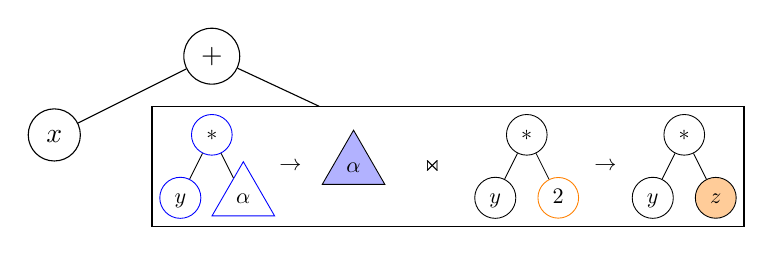
\begin{tikzpicture}
\node[varnode] (plus) {$+$};
\node[varnode] (x) at ($(plus)+(-2,-1)$) {$x$};
\node[changenode] (change) at ($(plus)+(3,-1.4)$) {\tikz{
    \node[varnode, color=blue] (del_times) {$\color{black}*$};
    \node[varnode, color=blue] (del_y) at ($(del_times)+(-0.5,-1)$) {$\color{black}y$};
    \node[mvnode, color=blue] (del_alpha) at ($(del_times)+(0.5,-1)$) {$\color{black}\alpha$};
    \draw (del_times) -- (del_y);
    \draw (del_times) -- (del_alpha);
    
    \node[mvnode, colorA] (ins_alpha) at ($(del_times)!0.5!(del_alpha)+(2, 0)$) {$\alpha$};
    \node (arrow) at ($(del_times)!0.5!(del_alpha)!0.5!(ins_alpha)$) {$\rightarrow$};
    
    \node[varnode] (odel_times) at ($(del_times)+(5,0)$) {$\color{black}*$};
    \node[varnode] (odel_y) at ($(odel_times)+(-0.5,-1)$) {$\color{black}y$};
    \node[varnode, color=orange] (odel_two) at ($(odel_times)+(0.5,-1)$) {$\color{black}2$};
    \draw (odel_times) -- (odel_y);
    \draw (odel_times) -- (odel_two);
    
    \node[varnode] (oins_times) at ($(odel_times)+(2.5, 0)$) {$*$};
    \node[varnode] (oins_y) at ($(oins_times)+(-0.5,-1)$) {$y$};
    \node[varnode, colorB] (oins_z) at ($(oins_times)+(0.5,-1)$) {$z$};
    \draw (oins_times) -- (oins_y);
    \draw (oins_times) -- (oins_z);
    
    \node (oarrow) at ($($(odel_times)!0.5!(odel_two)$)!0.5!($(oins_times)!0.5!(oins_y)$)$) {$\rightarrow$};
    
    \node (merge) at ($(ins_alpha)!0.5!($(odel_times)!0.5!(odel_y)$)$) {$\merge$};
}};
\draw (plus) -- (x);
\draw (plus) -- (change);
\end{tikzpicture}
\end{onlyenv}

\begin{onlyenv}<4>
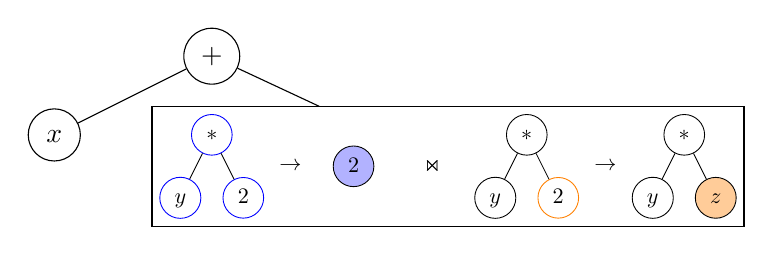
\begin{tikzpicture}
\node[varnode] (plus) {$+$};
\node[varnode] (x) at ($(plus)+(-2,-1)$) {$x$};
\node[changenode] (change) at ($(plus)+(3,-1.4)$) {\tikz{
    \node[varnode, color=blue] (del_times) {$\color{black}*$};
    \node[varnode, color=blue] (del_y) at ($(del_times)+(-0.5,-1)$) {$\color{black}y$};
    \node[varnode, color=blue] (del_alpha) at ($(del_times)+(0.5,-1)$) {$\color{black}2$};
    \draw (del_times) -- (del_y);
    \draw (del_times) -- (del_alpha);
    
    \node[varnode, colorA] (ins_alpha) at ($(del_times)!0.5!(del_alpha)+(2, 0)$) {$2$};
    \node (arrow) at ($(del_times)!0.5!(del_alpha)!0.5!(ins_alpha)$) {$\rightarrow$};
    
    \node[varnode] (odel_times) at ($(del_times)+(5,0)$) {$\color{black}*$};
    \node[varnode] (odel_y) at ($(odel_times)+(-0.5,-1)$) {$\color{black}y$};
    \node[varnode, color=orange] (odel_two) at ($(odel_times)+(0.5,-1)$) {$\color{black}2$};
    \draw (odel_times) -- (odel_y);
    \draw (odel_times) -- (odel_two);
    
    \node[varnode] (oins_times) at ($(odel_times)+(2.5, 0)$) {$*$};
    \node[varnode] (oins_y) at ($(oins_times)+(-0.5,-1)$) {$y$};
    \node[varnode, colorB] (oins_z) at ($(oins_times)+(0.5,-1)$) {$z$};
    \draw (oins_times) -- (oins_y);
    \draw (oins_times) -- (oins_z);
    
    \node (oarrow) at ($($(odel_times)!0.5!(odel_two)$)!0.5!($(oins_times)!0.5!(oins_y)$)$) {$\rightarrow$};
    
    \node (merge) at ($(ins_alpha)!0.5!($(odel_times)!0.5!(odel_y)$)$) {$\merge$};
}};
\draw (plus) -- (x);
\draw (plus) -- (change);
\end{tikzpicture}
\end{onlyenv}

\begin{onlyenv}<5>
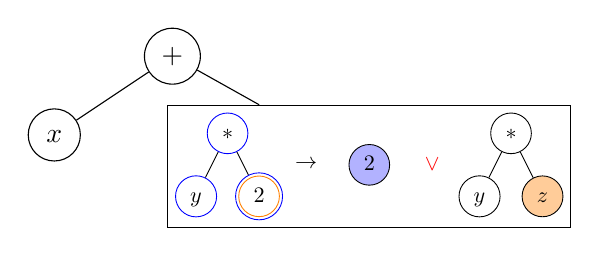
\begin{tikzpicture}
\node[varnode] (plus) {$+$};
\node[varnode] (x) at ($(plus)+(-1.5,-1)$) {$x$};
\node[changenode] (change) at ($(plus)+(2.5,-1.4)$) {\tikz{
    \node[varnode, color=blue] (del_times) {$\color{black}*$};
    \node[varnode, color=blue] (del_y) at ($(del_times)+(-0.5,-1)$) {$\color{black}y$};
    \node[varnode, color=orange] (del_alpha) at ($(del_times)+(0.5,-1)$) {$\color{black}2$};
    \node[varnode, color=blue] (del_alpha_out) at (del_alpha) {\phantom{M}};
    \draw (del_times) -- (del_y);
    \draw (del_times) -- (del_alpha_out);
    
    \node[varnode, colorA] (ins_alpha) at ($(del_times)!0.5!(del_alpha)+(2, 0)$) {$2$};
    \node (arrow) at ($(del_times)!0.5!(del_alpha)!0.5!(ins_alpha)$) {$\rightarrow$};
        
    \node[varnode] (oins_times) at ($(del_times)+(4.5, 0)$) {$*$};
    \node[varnode] (oins_y) at ($(oins_times)+(-0.5,-1)$) {$y$};
    \node[varnode, colorB] (oins_z) at ($(oins_times)+(0.5,-1)$) {$z$};
    \draw (oins_times) -- (oins_y);
    \draw (oins_times) -- (oins_z);
        
    \node (merge) at ($(ins_alpha)!0.5!($(oins_times)!0.5!(oins_y)$)$) {$\color{red}\vee$};
}};
\draw (plus) -- (x);
\draw (plus) -- (change);
\end{tikzpicture}
\end{onlyenv}
\end{frame}

\begin{frame}{Merging syntactic differences: Inline inside meta-variables}
\centering
\alt<2->{\tikzstyle{after2} = []}{\tikzstyle{after2} = [opacity=0]}
\alt<3->{\tikzstyle{after3} = []}{\tikzstyle{after3} = [opacity=0]}
\begin{onlyenv}<1-3>
\begin{tikzpicture}
    \node[varnode, color=blue] (adel_plus) {$\color{black}+$};
    \node[varnode, color=blue] (adel_three) at ($(adel_plus)+(-0.75,-1)$) {$\color{black}3$};
    \node[mvnode, color=blue] (adel_alpha) at ($(adel_plus)+(0.75,-1)$) {$\color{black}\alpha$};
    \draw (adel_plus) -- (adel_three);
    \draw (adel_plus) -- (adel_alpha);

    \node[varnode, colorA] (ains_minus) at ($(adel_plus)+(3.5,0)$) {$-$};
    \node[varnode, colorA] (ains_two) at ($(ains_minus)+(-0.75,-1)$) {$2$};
    \node[mvnode, colorA] (ains_alpha) at ($(ains_minus)+(0.75,-1)$) {$\alpha$};
    \draw (ains_minus) -- (ains_two);
    \draw (ains_minus) -- (ains_alpha);

    \node (aarrow) at ($($(adel_alpha)!0.5!(adel_plus)$)!0.5!($(ains_two)!0.5!(ains_minus)$)$) {$\rightarrow$};
    
    \node[varnode] (bdel_plus) at ($(adel_plus)+(0,-3)$) {$+$};
    \node[varnode] (bdel_three) at ($(bdel_plus)+(-0.75,-1)$) {$3$};
    \node[varnode, color=orange] (bdel_x) at ($(bdel_plus)+(0.75,-1)$) {$\color{black}x$};
    \draw (bdel_plus) -- (bdel_three);
    \draw (bdel_plus) -- (bdel_x);

    \node[varnode] (bins_plus) at ($(bdel_plus)+(3.5,0)$) {$+$};
    \node[varnode] (bins_three) at ($(bins_plus)+(-0.75,-1)$) {$3$};
    \node[varnode, colorB] (bins_times) at ($(bins_plus)+(0.75,-1)$) {$*$};
    \node[varnode, colorB] (bins_four) at ($(bins_times)+(-0.5,-1)$) {$4$};
    \node[mvnode, colorB] (bins_beta) at ($(bins_times)+(0.5,-1)$) {$\beta$};
    \node[mvnode, dotted, minimum size=3.5cm, color=blue,after2] (bins_alpha) at ($(bins_times)+(0,-0.75)$) {};
    \draw (bins_plus) -- (bins_three);
    \draw (bins_plus) -- (bins_times);
    \draw (bins_times) -- (bins_four);
    \draw (bins_times) -- (bins_beta);
    
    \node (barrow) at ($($(bdel_x)!0.5!(bdel_plus)$)!0.5!($(bins_three)!0.5!(bins_plus)$)$) {$\rightarrow$};
    
    \draw[>=latex,->,after2] ($(bins_plus)+(-0.75, 0.25)$) -- ($(adel_alpha)+(0, -0.5)$);
    \draw[->,dotted,after3] ($(ains_two)+(0, -0.5)$) -- ($(bdel_plus)+(0.75, 0.25)$);
\end{tikzpicture}
\end{onlyenv}

\begin{onlyenv}<4>
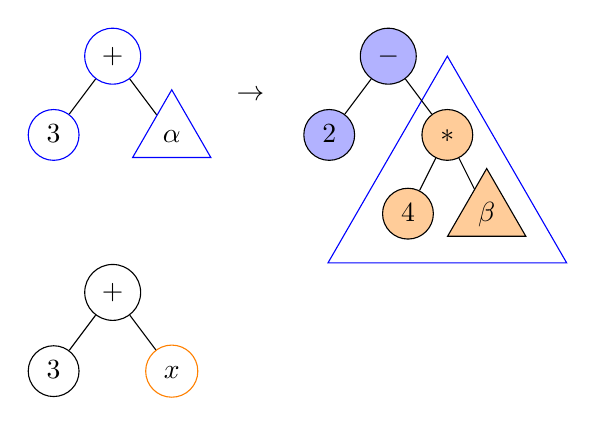
\begin{tikzpicture}
    \node[varnode, color=blue] (adel_plus) {$\color{black}+$};
    \node[varnode, color=blue] (adel_three) at ($(adel_plus)+(-0.75,-1)$) {$\color{black}3$};
    \node[mvnode, color=blue] (adel_alpha) at ($(adel_plus)+(0.75,-1)$) {$\color{black}\alpha$};
    \draw (adel_plus) -- (adel_three);
    \draw (adel_plus) -- (adel_alpha);

    \node[varnode] (bdel_plus) at ($(adel_plus)+(0,-3)$) {$+$};
    \node[varnode] (bdel_three) at ($(bdel_plus)+(-0.75,-1)$) {$3$};
    \node[varnode, color=orange] (bdel_x) at ($(bdel_plus)+(0.75,-1)$) {$\color{black}x$};
    \draw (bdel_plus) -- (bdel_three);
    \draw (bdel_plus) -- (bdel_x);

    \node[varnode, colorA] (ins_minus) at ($(adel_plus)+(3.5,0)$) {$-$};
    \node[varnode, colorA] (ins_two) at ($(ins_minus)+(-0.75,-1)$) {$2$};
    \node[varnode, colorB] (ins_times) at ($(ins_minus)+(0.75,-1)$) {$*$};
    \node[varnode, colorB] (ins_four) at ($(ins_times)+(-0.5,-1)$) {$4$};
    \node[mvnode, colorB] (ins_beta) at ($(ins_times)+(0.5,-1)$) {$\beta$};
    \node[mvnode, minimum size=3.5cm, color=blue] (ins_alpha) at ($(ins_times)+(0,-0.75)$) {};
    \draw (ins_minus) -- (ins_two);
    \draw (ins_minus) -- (ins_times);
    \draw (ins_times) -- (ins_four);
    \draw (ins_times) -- (ins_beta);

    \node (arrow) at ($($(adel_alpha)!0.5!(adel_plus)$)!0.5!($(ins_two)!0.5!(ins_minus)$)$) {$\rightarrow$};
\end{tikzpicture}
\end{onlyenv}


\begin{onlyenv}<5>
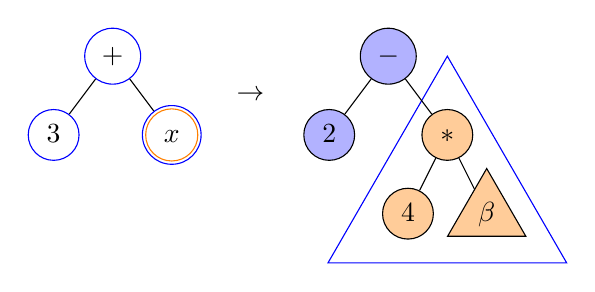
\begin{tikzpicture}
    \node[varnode, color=blue] (del_plus) {$\color{black}+$};
    \node[varnode, color=blue] (del_three) at ($(del_plus)+(-0.75,-1)$) {$\color{black}3$};
    \node[varnode, color=orange] (del_x) at ($(del_plus)+(0.75,-1)$) {$\color{black}x$};
    \node[varnode, color=blue] (del_x_out) at (del_x) {\phantom{M}};
    \draw (del_plus) -- (del_three);
    \draw (del_plus) -- (del_x_out);

    \node[varnode, colorA] (ins_minus) at ($(del_plus)+(3.5,0)$) {$-$};
    \node[varnode, colorA] (ins_two) at ($(ins_minus)+(-0.75,-1)$) {$2$};
    \node[varnode, colorB] (ins_times) at ($(ins_minus)+(0.75,-1)$) {$*$};
    \node[varnode, colorB] (ins_four) at ($(ins_times)+(-0.5,-1)$) {$4$};
    \node[mvnode, colorB] (ins_beta) at ($(ins_times)+(0.5,-1)$) {$\beta$};
    \node[mvnode, minimum size=3.5cm, color=blue] (ins_alpha) at ($(ins_times)+(0,-0.75)$) {};
    \draw (ins_minus) -- (ins_two);
    \draw (ins_minus) -- (ins_times);
    \draw (ins_times) -- (ins_four);
    \draw (ins_times) -- (ins_beta);

    \node (arrow) at ($($(del_x)!0.5!(del_plus)$)!0.5!($(ins_two)!0.5!(ins_minus)$)$) {$\rightarrow$};
\end{tikzpicture}
\end{onlyenv}
\end{frame}

\begin{frame}{Merging syntactic differences: Principles and advancement}
\begin{block}{Theoretical guarantees wanted}
 \begin{itemize}
  \item No change is ever lost
  \item Commutative ($t \merge u = u \merge t$)
  \item Idempotent ($t \merge t = t$)
  \item Identity is neutral ($t \merge id = t$)
  \item Intersect domains ($\dom(t \merge u) \supseteq \dom(t) \cap \dom(u)$)
  \item Compatible with composition and inverse
 \end{itemize}
\end{block}

\begin{exampleblock}<2->{Work achieved}
 \begin{itemize}
  \item Manual quadratic effort
  \item Implementation that works on examples ($\approx 5000$ LoC)
  \item Work in progress formal specification
  \item No proof of correctness yet
 \end{itemize}
\end{exampleblock}
\end{frame}


\begin{frame}[fragile]{Merging syntactic differences: Example}
\begin{columns}
\begin{column}{0.33\textwidth}
\setstcolor{blue}
\setulcolor{blue}
\newbox\boxsemicolon
\sbox\boxsemicolon{\color{blue}\scriptsize\ttfamily;}
\center{\color{blue}Blue difference}
\vspace{0.5em}
\begin{lstlisting}[rulecolor=\color{blue!20}]
fn f(c: bool) -> i32 {
    @\st{$\alpha$;}@
    @\st{$\beta$;}@
    let x = @\st{$\gamma$} $\rightarrow$@
        @{\color{blue}\ul{answer()}}@;
    let y = if @$\id$@ {
        @$\id$@;
    } else {
        @\st{$\delta$} $\rightarrow$ \ul{$\delta$ {\color{blue}*} $\delta$}@
    };
    @\st{$\delta$ * $\epsilon$} $\rightarrow$ \ul{$\delta$ {\color{blue}/} $\epsilon$}@
}

@{\color{blue} \ul{fn answer() -> i32 \{}}@
    @\ul{$\alpha${\usebox\boxsemicolon}}@
    @\ul{$\beta${\usebox\boxsemicolon}}@
    @\ul{$\gamma$}@
@{\color{blue} \ul{\}}}@
\end{lstlisting}
\end{column}
\begin{column}{0.33\textwidth}
\newbox\boxtwo
\sbox\boxtwo{\setulcolor{orange}\setul{-.75ex}{}\ul{\scriptsize\ttfamily 2}}
\newbox\boxforty
\sbox\boxforty{\setulcolor{orange}\setul{-.75ex}{}\ul{\scriptsize\ttfamily 40}}
\center{Merged difference}
\vspace{0.5em}
\begin{onlyenv}<1>
\begin{lstlisting}
fn f(c: bool) -> i32 {
    @\setstcolor{blue}\st{let a = {\usebox\boxtwo};}@
    @\setstcolor{blue}\st{let b = {\usebox\boxforty};}@
    let x = @\setstcolor{blue}\st{a + b}@ @$\rightarrow$@
        @{\color{blue}\ul{answer()}}@;
    let y = if @$\square$@ {
        @\setstcolor{orange}\st{2} $\rightarrow$ {\color{orange}\ul{0}}@
    } else {
        @\setstcolor{blue}\st{$\delta$} $\rightarrow$ \setulcolor{blue}\ul{$\delta$ {\color{blue}*} $\delta$}@
    };
    @\setstcolor{blue}\st{$\delta$ * $\epsilon$} $\rightarrow$ \setulcolor{blue}\ul{$\delta$ {\color{blue}/} $\epsilon$}@
}

@{\color{blue}\ul{fn answer() -> i32 \{}}@
    @\setulcolor{blue}\ul{let a = {\color{orange}4};}@
    @\setulcolor{blue}\ul{let b = {\color{orange}41};}@
    @\setulcolor{blue}\ul{a + b}@
@{\color{blue}\ul{\}}}@
\end{lstlisting}
\end{onlyenv}%
\begin{onlyenv}<2>
\begin{lstlisting}
fn f(c: bool) -> i32 {
    @\setstcolor{blue}\st{let a = {\usebox\boxtwo};}@
    @\setstcolor{blue}\st{let b = {\usebox\boxforty};}@
    let x = @\setstcolor{blue}\st{a + b}@ @$\rightarrow$@
        @{\color{blue}\ul{answer()}}@;
    let y = if c {
        @\setstcolor{orange}\st{2} $\rightarrow$ {\color{orange}\ul{0}}@
    } else {
        @\setstcolor{blue}\st{x} $\rightarrow$ \setulcolor{blue}\ul{x {\color{blue}*} x}@
    };
    @\setstcolor{blue}\st{x * y} $\rightarrow$ \setulcolor{blue}\ul{x {\color{blue}/} y}@
}

@{\color{blue}\ul{fn answer() -> i32 \{}}@
    @\setulcolor{blue}\ul{let a = {\color{orange}4};}@
    @\setulcolor{blue}\ul{let b = {\color{orange}41};}@
    @\setulcolor{blue}\ul{a + b}@
@{\color{blue}\ul{\}}}@
\end{lstlisting}
\end{onlyenv}
\end{column}
\begin{column}{.33\textwidth}
\setstcolor{orange}
\setulcolor{orange}
\center{\color{orange}Orange difference}
\vspace{0.5em}
\begin{lstlisting}[rulecolor=\color{orange!30}]
fn f(c: bool) -> i32 {
    let a = @\st{2} $\rightarrow$ {\color{orange}\ul{4}}@;
    let b = @\st{40} $\rightarrow$ {\color{orange}\ul{41}}@;
    @$\id$@;

    let y = if @$\id$@ {
        @\st{2} $\rightarrow$ {\color{orange}\ul{0}}@
    } else {
        @$\id$@
    };
    @$\id$@
}





@@
\end{lstlisting}
\end{column}
\end{columns}
\end{frame}

\section{Semantic check}
\sectiontitleframe

\begin{frame}[fragile]{Semantic check}
\begin{alertblock}{Goal}
Check that no commit rely on invariants broken by another commit
\end{alertblock}

\begin{exampleblock}{Example: Double fix}
\begin{onlyenv}<-3>
\begin{lstlisting}
fn compute_something(x: i32) -> i32 {
    let mut a = x * x;
    @\color{blue}\ul{a += 1;}@
    @\setstcolor{orange}\st{a} $\rightarrow$ {\color{orange}\ul{a + 1}}@
}
\end{lstlisting}
\end{onlyenv}
\begin{onlyenv}<4>
\begin{lstlisting}
fn f() -> bool {
    let mut res = @\setstcolor{orange}\st{true} $\rightarrow$ {\color{orange}\ul{false}}@;
    @\setstcolor{blue}\st{res = !res;}@
    res
}
\end{lstlisting}
\end{onlyenv}
\end{exampleblock}

\begin{block}<2->{Principles}
\begin{itemize}
 \item<2-> Runtime analysis (for now)
 \item<3-> Propagate colors in runtime values
 \item<4-> Interleave execution of original and merged code
\end{itemize}
\end{block}
\end{frame}

\begin{frame}[fragile]{Correlation oracle}
\begin{columns}
\begin{column}{0.33\textwidth}
\center{\color{red}Original}
\vspace{0.5em}
\begin{lstlisting}[rulecolor=\color{red!20}]
fn f(c: bool) -> i32 {@\only<1>{\color{red}$\bullet$}@
    let w = 40;@\only<2>{\color{red}$\bullet$}@
    let x = 2 + w;@\only<3-4>{\color{red}$\bullet$}@
    
    let y = if c@\alt<5>{\color{red}$\bullet$}{ }@{
        2
    } else {
        x@\only<6-7>{\color{red}$\bullet$}@
    };@\only<8>{\color{red}$\bullet$}@
    x * y@\only<9>{\color{red}$\bullet$}@
}
\end{lstlisting}
\end{column}
\begin{column}{0.33\textwidth}
\center{Difference}
\vspace{0.5em}
\begin{lstlisting}
fn f(c: bool) -> i32 {@\only<1>{$\bullet$}@
    @\color{red}\st{let w = 40;}@@\only<2>{$\bullet$}@
    let x = @\color{red}\st{2+w}@ @$\rightarrow$@ @{\color{olive}\ul{42}}@;@\only<3>{$\bullet$}@
    @\color{olive}\ul{let z = !c;}@@\only<4>{$\bullet$}@
    let y = if @\color{red}\st{c}@ @$\rightarrow$@ @{\color{olive}\ul{z}}\alt<5-6>{\only<6>{\color{olive}}$\bullet$}{ }@{
        @{\color{red}\st{2}} $\rightarrow$ {\color{olive}\ul{1}}\only<7>{\color{olive}$\bullet$}@
    } else {
        @{\color{red}\st{x}} $\rightarrow$ {\color{olive}\ul{x * x}}\only<6-7>{\color{red}$\bullet$}@
    };@\only<8>{$\bullet$}@
    x * y@\only<9>{$\bullet$}@
}
\end{lstlisting}
\end{column}
\begin{column}{0.33\textwidth}
\center{\color{olive}Modified}
\vspace{0.5em}
\begin{lstlisting}[rulecolor=\color{olive!20}]
fn f(c: bool) -> i32 {@\only<1-2>{\color{olive}$\bullet$}@
    
    let x = 42;@\only<3>{\color{olive}$\bullet$}@
    let z = !c;@\only<4>{\color{olive}$\bullet$}@
    let y = if z@\alt<5-6>{\color{olive}$\bullet$}{ }@{
        1@\only<7>{\color{olive}$\bullet$}@
    } else {
        x * x
    };@\only<8>{\color{olive}$\bullet$}@
    x * y@\only<9>{\color{olive}$\bullet$}@
}
\end{lstlisting}
\end{column}
\end{columns}
\setstcolor{red}\setulcolor{olive}
\begin{center}
\alt<1>{\tikzstyle{hl1} = [opacity=1]}{\tikzstyle{hl1} = []}
\alt<2>{\tikzstyle{hl2} = [opacity=1]}{\tikzstyle{hl2} = []}
\alt<3>{\tikzstyle{hl3} = [opacity=1]}{\tikzstyle{hl3} = []}
\alt<4>{\tikzstyle{hl4} = [opacity=1]}{\tikzstyle{hl4} = []}
\alt<5>{\tikzstyle{hl5} = [opacity=1]}{\tikzstyle{hl5} = []}
\alt<6>{\tikzstyle{hl6} = [opacity=1]}{\tikzstyle{hl6} = []}
\alt<7>{\tikzstyle{hl7} = [opacity=1]}{\tikzstyle{hl7} = []}
\alt<8>{\tikzstyle{hl8} = [opacity=1]}{\tikzstyle{hl8} = []}
\alt<9>{\tikzstyle{hl9} = [opacity=1]}{\tikzstyle{hl9} = []}
\begin{tikzpicture}
    \node[opacity=0.6, hl1] (o1) {1};
    \node[right of=o1, opacity=0.6, hl2] (o2) {\st{2}};
    \node[right of=o2, opacity=0.6, hl3] (o3) {3};
    \node[right of=o3, opacity=0.6, hl4] (o4) {\ul{4}};
    \node[right of=o4, opacity=0.6, hl5] (o5) {5};
    \node[right of=o5, opacity=0.6, hl6] (o8) {\st{8}};
    \node[right of=o8, opacity=0.6, hl7] (o6) {\ul{6}};
    \node[right of=o6, opacity=0.6, hl8] (o9) {9};
    \node[right of=o9, opacity=0.6, hl9] (o10) {10};
    \draw[->] (o1) -- (o2);
    \draw[->] (o2) -- (o3);
    \draw[->] (o3) -- (o4);
    \draw[->] (o4) -- (o5);
    \draw[->] (o5) -- (o8);
    \draw[->] (o8) -- (o6);
    \draw[->] (o6) -- (o9);
    \draw[->] (o9) -- (o10);

    \node[red, above of=o1, opacity=0.6, hl1] (d1) {1};
    \node[red, above of=o2, opacity=0.6, hl2] (d2) {2};
    \node[red, above of=o3, opacity=0.6, hl3, hl4] (d3) {3};
    \node[red, above of=o5, opacity=0.6, hl5] (d5) {5};
    \node[red, above of=o8, opacity=0.6, hl6, hl7] (d8) {8};
    \node[red, above of=o9, opacity=0.6, hl8] (d9) {9};
    \node[red, above of=o10, opacity=0.6, hl9] (d10) {10};
    \draw[red, ->] (d1) -- (d2);
    \draw[red, ->] (d2) -- (d3);
    \draw[red, ->] (d3) -- (d5);
    \draw[red, ->] (d5) -- (d8);
    \draw[red, ->] (d8) -- (d9);
    \draw[red, ->] (d9) -- (d10);
    \draw[dotted, ->] (o1) -- (d1);
    \draw[dotted, ->] (o2) -- (d2);
    \draw[dotted, ->] (o3) -- (d3);
    \draw[dotted, ->] (o4) -- (d3);
    \draw[dotted, ->] (o5) -- (d5);
    \draw[dotted, ->] (o8) -- (d8);
    \draw[dotted, ->] (o6) -- (d8);
    \draw[dotted, ->] (o9) -- (d9);
    \draw[dotted, ->] (o10) -- (d10);

    \node[olive, below of=o1, opacity=0.6, hl1, hl2] (i1) {1};
    \node[olive, below of=o3, opacity=0.6, hl3] (i3) {3};
    \node[olive, below of=o4, opacity=0.6, hl4] (i4) {4};
    \node[olive, below of=o5, opacity=0.6, hl5, hl6] (i5) {5};
    \node[olive, below of=o6, opacity=0.6, hl7] (i6) {6};
    \node[olive, below of=o9, opacity=0.6, hl8] (i9) {9};
    \node[olive, below of=o10, opacity=0.6, hl9] (i10) {10};
    \draw[olive, ->] (i1) -- (i3);
    \draw[olive, ->] (i3) -- (i4);
    \draw[olive, ->] (i4) -- (i5);
    \draw[olive, ->] (i5) -- (i6);
    \draw[olive, ->] (i6) -- (i9);
    \draw[olive, ->] (i9) -- (i10);
    \draw[dotted, ->] (o1) -- (i1);
    \draw[dotted, ->] (o2) -- (i1);
    \draw[dotted, ->] (o3) -- (i3);
    \draw[dotted, ->] (o4) -- (i4);
    \draw[dotted, ->] (o5) -- (i5);
    \draw[dotted, ->] (o8) -- (i5);
    \draw[dotted, ->] (o6) -- (i6);
    \draw[dotted, ->] (o9) -- (i9);
    \draw[dotted, ->] (o10) -- (i10);
\end{tikzpicture}
\end{center}
\end{frame}

\begin{frame}[fragile]{Colored correlation oracle}
\begin{onlyenv}<1>
\begin{columns}
\begin{column}{0.45\textwidth}
\begin{lstlisting}
let mut res = @\setstcolor{orange}\st{true} $\rightarrow$ {\color{orange}\ul{false}}@;
@\setstcolor{blue}\st{res = !res;}@
res
\end{lstlisting}
\end{column}
\begin{column}{0.45\textwidth}
\begin{align*}
\square &\mapsto ()\\
\end{align*}
\end{column}
\end{columns}
\end{onlyenv}

\begin{onlyenv}<2>
\begin{columns}
\begin{column}{0.45\textwidth}
\begin{lstlisting}
@\setstcolor{orange}\st{true}@
@{\color{orange}\ul{false}}@
let mut res = @$\square$@;
@\setstcolor{blue}\st{res = !res;}@
res
\end{lstlisting}
\end{column}
\begin{column}{0.45\textwidth}
\begin{align*}
\square &\mapsto ()\\
\end{align*}
\end{column}
\end{columns}
\end{onlyenv}

\begin{onlyenv}<3>
\begin{columns}
\begin{column}{0.45\textwidth}
\begin{lstlisting}
@{\color{orange}\ul{false}}@
let mut res = @$\square$@;
@\setstcolor{blue}\st{res = !res;}@
res
\end{lstlisting}
\end{column}
\begin{column}{0.45\textwidth}
\begin{align*}
\square &\mapsto \color{orange}\mathst{true}, \mathul{()}\\
\end{align*}
\end{column}
\end{columns}
\end{onlyenv}

\begin{onlyenv}<4>
\begin{columns}
\begin{column}{0.45\textwidth}
\begin{lstlisting}
let mut res = @$\square$@;
@\setstcolor{blue}\st{res = !res;}@
res
\end{lstlisting}
\end{column}
\begin{column}{0.45\textwidth}
\begin{align*}
\square &\mapsto \color{orange}\mathst{true}, \mathul{false}\\
\end{align*}
\end{column}
\end{columns}
\end{onlyenv}

\begin{onlyenv}<5>
\begin{columns}
\begin{column}{0.45\textwidth}
\begin{lstlisting}
@\setstcolor{blue}\st{res = !res;}@
res
\end{lstlisting}
\end{column}
\begin{column}{0.45\textwidth}
\begin{align*}
\square &\mapsto ()\\
res &\mapsto \color{orange}\mathst{true}, \mathul{false}\\
\end{align*}
\end{column}
\end{columns}
\end{onlyenv}

\begin{onlyenv}<6>
\begin{columns}
\begin{column}{0.45\textwidth}
\begin{lstlisting}
@\setstcolor{blue}\st{!res}@
@\setstcolor{blue}\st{res = $\square$;}@
res
\end{lstlisting}
\end{column}
\begin{column}{0.45\textwidth}
\begin{align*}
\square &\mapsto ()\\
res &\mapsto \color{orange}\mathst{true}, \mathul{false}\\
\end{align*}
\end{column}
\end{columns}
\end{onlyenv}

\begin{onlyenv}<7>
\begin{columns}
\begin{column}{0.45\textwidth}
\begin{lstlisting}
@\setstcolor{blue}\st{res}@
@\setstcolor{blue}\st{!$\square$}@
@\setstcolor{blue}\st{res = $\square$;}@
res
\end{lstlisting}
\end{column}
\begin{column}{0.45\textwidth}
\begin{align*}
\square &\mapsto ()\\
res &\mapsto \color{orange}\mathst{true}, \mathul{false}\\
\end{align*}
\end{column}
\end{columns}
\end{onlyenv}

\begin{onlyenv}<8>
\begin{columns}
\begin{column}{0.45\textwidth}
\begin{lstlisting}
@\setstcolor{blue}\st{!$\square$}@
@\setstcolor{blue}\st{res = $\square$;}@
res
\end{lstlisting}
\end{column}
\begin{column}{0.45\textwidth}
\begin{align*}
\square &\mapsto \color{blue}\mathst{true}, \mathul{()}\\
res &\mapsto \color{orange}\mathst{true}, \mathul{false}\\
\end{align*}
\end{column}
\end{columns}
\end{onlyenv}

\begin{onlyenv}<9>
\begin{columns}
\begin{column}{0.45\textwidth}
\begin{lstlisting}
@\setstcolor{blue}\st{res = $\square$;}@
res
\end{lstlisting}
\end{column}
\begin{column}{0.45\textwidth}
\begin{align*}
\square &\mapsto \color{blue}\mathst{false}, \mathul{()}\\
res &\mapsto \color{orange}\mathst{true}, \mathul{false}\\
\end{align*}
\end{column}
\end{columns}
\end{onlyenv}

\begin{onlyenv}<10>
\begin{columns}
\begin{column}{0.45\textwidth}
\begin{lstlisting}
res
\end{lstlisting}
\end{column}
\begin{column}{0.45\textwidth}
\newbox\boxresval
\sbox\boxresval{$\color{white}\mathst{false}, \mathul{false}$}
\begin{align*}
\square &\mapsto ()\\
res &\mapsto \black{\usebox\boxresval}\\
\end{align*}

Semantic ambiguity found !
\end{column}
\end{columns}
\end{onlyenv}
\end{frame}

\begin{frame}[fragile]{Colored correlation oracle: control flow}
\begin{onlyenv}<1>
\begin{columns}
\begin{column}{0.45\textwidth}
\begin{lstlisting}
let y = if @\setstcolor{orange}\st{c}@ @$\rightarrow$@ @{\color{orange}\ul{!c}}@ {
    @{\setstcolor{orange}\st{2}} $\rightarrow$ {\color{orange}\ul{1}}@
} else {
    @{\setstcolor{blue}\st{x}} $\rightarrow$ {\color{blue}\ul{x * x}}@
};
x * y
\end{lstlisting}
\end{column}
\begin{column}{0.45\textwidth}
\begin{align*}
\square &\mapsto ()\\
x &\mapsto 3\\
c &\mapsto true\\
\end{align*}
\end{column}
\end{columns}
\end{onlyenv}

\begin{onlyenv}<2>
\begin{columns}
\begin{column}{0.45\textwidth}
\begin{lstlisting}
@\setstcolor{orange}\st{c}@
@\color{orange}\ul{!c}@
if @$\square$@ {
    @{\setstcolor{orange}\st{2}} $\rightarrow$ {\color{orange}\ul{1}}@
} else {
    @{\setstcolor{blue}\st{x}} $\rightarrow$ {\color{blue}\ul{x * x}}@
}
let y = @$\square$@;
x * y
\end{lstlisting}
\end{column}
\begin{column}{0.45\textwidth}
\begin{align*}
\square &\mapsto ()\\
x &\mapsto 3\\
c &\mapsto true\\
\end{align*}
\end{column}
\end{columns}
\end{onlyenv}

\begin{onlyenv}<3>
\begin{columns}
\begin{column}{0.45\textwidth}
\begin{lstlisting}
if @$\square$@ {
    @{\setstcolor{orange}\st{2}} $\rightarrow$ {\color{orange}\ul{1}}@
} else {
    @{\setstcolor{blue}\st{x}} $\rightarrow$ {\color{blue}\ul{x * x}}@
}
let y = @$\square$@;
x * y
\end{lstlisting}
\end{column}
\begin{column}{0.45\textwidth}
\begin{align*}
\square &\mapsto \color{orange}\mathst{true}, \mathul{false}\\
x &\mapsto 3\\
c &\mapsto true\\
\end{align*}
\end{column}
\end{columns}
\end{onlyenv}

\begin{onlyenv}<4>
\begin{columns}
\begin{column}{0.45\textwidth}
\begin{lstlisting}
@\setstcolor{orange}\st{if $\square$ \{}@
    @\setstcolor{orange}\st{2}@
@\setstcolor{orange}\st{\} else \{}@
    @\st{x}@
@\setstcolor{orange}\st{\}}@
@\color{orange}\ul{if $\square$ \{}@
    @{\color{orange}\ul{1}}@
@\color{orange}\ul{\} else \{}@
    @{\color{blue}\setulcolor{orange}\ul{x * x}}@
@\color{orange}\ul{\}}@
let y = @$\square$@;
x * y
\end{lstlisting}
\end{column}
\begin{column}{0.45\textwidth}
\begin{align*}
\square &\mapsto \color{orange}\mathst{true}, \mathul{false}\\
x &\mapsto 3\\
c &\mapsto true\\
\end{align*}
\end{column}
\end{columns}
\end{onlyenv}

\begin{onlyenv}<5>
\begin{columns}
\begin{column}{0.45\textwidth}
\begin{lstlisting}
@\setstcolor{orange}\st{2}@
@\color{orange}\ul{if $\square$ \{}@
    @{\color{orange}\ul{1}}@
@\color{orange}\ul{\} else \{}@
    @{\color{blue}\setulcolor{orange}\ul{x * x}}@
@\color{orange}\ul{\}}@
let y = @$\square$@;
x * y
\end{lstlisting}
\end{column}
\begin{column}{0.45\textwidth}
\begin{align*}
\square &\mapsto \color{orange}\mathst{()}, \mathul{false}\\
x &\mapsto 3\\
c &\mapsto true\\
\end{align*}
\end{column}
\end{columns}
\end{onlyenv}

\begin{onlyenv}<6>
\begin{columns}
\begin{column}{0.45\textwidth}
\begin{lstlisting}
@\color{orange}\ul{if $\square$ \{}@
    @{\color{orange}\ul{1}}@
@\color{orange}\ul{\} else \{}@
    @{\color{blue}\setulcolor{orange}\ul{x * x}}@
@\color{orange}\ul{\}}@
let y = @$\square$@;
x * y
\end{lstlisting}
\end{column}
\begin{column}{0.45\textwidth}
\begin{align*}
\square &\mapsto \color{orange}\mathst{2}, \mathul{false}\\
x &\mapsto 3\\
c &\mapsto true\\
\end{align*}
\end{column}
\end{columns}
\end{onlyenv}

\begin{onlyenv}<7>
\begin{columns}
\begin{column}{0.45\textwidth}
\begin{lstlisting}
@{\color{blue}\setulcolor{orange}\ul{x * x}}@
let y = @$\square$@;
x * y
\end{lstlisting}
\end{column}
\begin{column}{0.45\textwidth}
\begin{align*}
\square &\mapsto \color{orange}\mathst{2}, \mathul{()}\\
x &\mapsto 3\\
c &\mapsto true\\
\end{align*}
\end{column}
\end{columns}
\end{onlyenv}

\begin{onlyenv}<8>
\begin{columns}
\begin{column}{0.45\textwidth}
\begin{lstlisting}
@{\color{blue}\setulcolor{orange}\ul{$\square$ * x}}@
let y = @$\square$@;
x * y
\end{lstlisting}
\end{column}
\begin{column}{0.45\textwidth}
\newbox\boxsquareval
\sbox\boxsquareval{$\color{white}\mathst{2}, \mathul{3}$}
\begin{align*}
\square &\mapsto \black{\usebox\boxsquareval}\\
x &\mapsto 3\\
c &\mapsto true\\
\end{align*}

Semantic ambiguity found !
\end{column}
\end{columns}
\end{onlyenv}

\end{frame}

\section{Resolving conflicts}
\sectiontitleframe

\begin{frame}[fragile]{Resolving conflicts}
\begin{columns}
\begin{column}{0.48\textwidth}
\begin{block}{Conflict resolution tactics}
Refine the merged program to resolve conflicts with tactics:
\begin{itemize}
 \item<2-> Declare semantic preserving change
 \item<3-> Revert a change
 \item<4-> Introduce new change
 \item<5-> Create reviewed interaction block
 \item<6-> Resolve syntactic conflicts
\end{itemize}

Rerun the semantic analysis between tactic applications
\end{block}
\end{column}
\begin{column}{0.48\textwidth}
\begin{exampleblock}{Example}
\begin{onlyenv}<-6>
\newbox\boxtwo
\sbox\boxtwo{\setulcolor{orange}\setul{-.75ex}{}\ul{\scriptsize\ttfamily 2}}
\newbox\boxforty
\sbox\boxforty{\setulcolor{orange}\setul{-.75ex}{}\ul{\scriptsize\ttfamily 40}}
\alt<1>{\def\spblue{blue}}{\def\spblue{black}}
\begin{lstlisting}
fn f(c: bool) -> i32 {
    @\setstcolor{\spblue}\st{let a = {\usebox\boxtwo};}@
    @\setstcolor{\spblue}\st{let b = {\usebox\boxforty};}@
    let x = @\setstcolor{\spblue}\st{a + b}@ @$\rightarrow$@
        @{\color{\spblue}\ul{answer()}}@;
    let y = if c {
        @\setstcolor{orange}\st{2} $\rightarrow$ {\color{orange}\ul{0}}@
    } else {
        @\setstcolor{blue}\st{x} $\rightarrow$ \setulcolor{blue}\ul{x {\color{blue}*} x}@
    };
    @\only<1-2>{\setstcolor{blue}\st{x * y} $\rightarrow$ \setulcolor{blue}\ul{x {\color{blue}/} y}}\only<3>{x * y}\only<4,6>{\st{x * y} $\rightarrow$ \ul{x / (y+1)}}\only<5>{reviewed \{ \setstcolor{blue}\st{x * y} $\rightarrow$ \setulcolor{blue}\ul{x {\color{blue}/} y} \}}@
}

@{\color{\spblue}\ul{fn answer() -> i32 \{}}@
    @\setulcolor{\spblue}\ul{let a = {\color{orange}4};}@
    @\setulcolor{\spblue}\ul{let b = {\color{orange}41};}@
    @\setulcolor{\spblue}\ul{a + b}@
@{\color{\spblue}\ul{\}}}@
\end{lstlisting}
\end{onlyenv}
\begin{onlyenv}<7>
\begin{lstlisting}
fn f(c: bool) -> i32 {
    let x = answer();
    let y = if c {
        @\color{orange}0@
    } else {
        @\color{blue}x * x@
    };
    @\ul{x / (y+1)}@
}

fn answer() -> i32 {
    let a = @\color{orange}4@;
    let b = @\color{orange}41@;
    a + b
}
\end{lstlisting}
\end{onlyenv}
\end{exampleblock}
\end{column}
\end{columns}
\end{frame}

\section*{Conclusion}
\begin{frame}{Conclusion}
\begin{block}{Contributions}
\begin{itemize}
 \item Syntactic fusion of source code change tracking provenance
 \item<2-> Implementation of the merging algorithm in Rust
 \item<3-> Framework for a semantic analysis tracking interactions
 \item<4-> Interactive conflict resolution
\end{itemize}
\end{block}
\begin{exampleblock}{Future works}
\begin{itemize}
 \item<5-> More theoretical guarantees for syntactic fusion
 \item<6-> Combine our semantic analysis with static analysis or fuzzing techniques
 \item<7-> Implement the semantic check phase
 \item<8-> Design more automated resolution tactics
 \item<9-> Test on real projects / adapt on other languages
\end{itemize}
\end{exampleblock}
\end{frame}


\end{document}
